\documentclass[uplatex,dvipdfmx,a4paper,11pt]{jsarticle}

\usepackage[top=25mm,bottom=25mm,left=25mm,right=25mm]{geometry}

\usepackage{array}
\usepackage{tabularx}
\usepackage{booktabs}
\usepackage{enumitem}
\usepackage{graphicx}

\setlength{\parindent}{0pt}
\setlength{\parskip}{0.6em}

\usepackage{titlesec}
\titleformat{\section}
  {\normalfont\Large\bfseries}{\thesection.}{0.6em}{}
\titleformat{\subsection}
  {\normalfont\large\bfseries}{\thesubsection}{0.6em}{}
\titlespacing*{\section}{0pt}{1.2em}{0.6em}
\titlespacing*{\subsection}{0pt}{1.0em}{0.4em}

\newcommand{\sectionrule}{\par\medskip\noindent\rule{\linewidth}{0.6pt}\par\medskip}

\renewcommand{\labelitemi}{\textbullet}
\renewcommand{\labelitemii}{\textopenbullet}
\setlist[itemize]{leftmargin=1.6em,itemsep=0.1em,topsep=0.2em}
\setlist[enumerate]{leftmargin=2.0em,itemsep=0.1em,topsep=0.2em}

\providecommand{\textopenbullet}{\ensuremath{\circ}}

\begin{document}

{\LARGE\bfseries 作業ログ}\par\bigskip

報告者：齋藤　翔太

報告日：2026年6月16日

プロジェクト名：タクトーン〜IMUジェスチャーで奏でるArduinoオーケストラ〜

\sectionrule

\section{進捗サマリー（要約）}

\begin{itemize}
  \item 全体進捗率：98％
  \item マイルストーン達成状況：予定通り進行中
  \item 主要成果：
    \begin{itemize}
      \item {}音声分析プログラムの再構築を行なった．
      \item {}金管楽器の音色の再分析と作成を完了した．
      \item {}ドラムの音色の分析と作成を完了した．
      \item {}トランペット音色の比較調整を行いやすくするため，A/B比較機能，直接数値入力，調整プリセットを追加した．
    \end{itemize}
  \item 重大課題（影響度：高）：
    \begin{itemize}
      \item {}なし
    \end{itemize}
\end{itemize}

\sectionrule

\section{作業ログ（詳細トラッキング）}

{\footnotesize
\renewcommand{\arraystretch}{1.25}
\begin{tabularx}{\linewidth}{@{}>{\raggedright\arraybackslash}p{21mm}>{\raggedright\arraybackslash}p{13mm}>{\raggedright\arraybackslash}p{17mm}>{\raggedright\arraybackslash}p{16mm}>{\raggedright\arraybackslash}p{12mm}XX@{}}
\toprule
作業項目 & 開始日 & 予定完了日 & 状態 & 進捗率 & 依存関係・ブロッカー & コメント \\
\midrule
音色の分析プログラムの再構築
  & 6/10 & 6/10 & 完了 & 100\%
  & なし
  & 音声解析プログラムの改善を行なった．\\
金管楽器の音色の再分析と作成
  & 6/10 & 6/16 & 完了 & 100\%
  & なし
  & 金管楽器の音色の再分析と作成を完了した．\\
ドラムの音色の分析と作成
  & 6/12 & 6/12 & 完了 & 100\%
  & なし
  & ドラムの音色の分析と作成を完了した．\\
トランペット音色調整UIの改良
  & 6/16 & 6/16 & 完了 & 100\%
  & なし
  & A/B比較機能，調整プリセット，数値直接入力欄を追加し，試聴しながら調整しやすくした．\\
\bottomrule
\end{tabularx}
}

\newpage
\subsection{日ごとの作業時間・作業内容}

{\footnotesize
\renewcommand{\arraystretch}{1.25}
\begin{tabularx}{\linewidth}{@{}>{\raggedright\arraybackslash}p{16mm}>{\raggedright\arraybackslash}p{22mm}XX@{}}
\toprule
日付 & 作業時間 & 作業内容 & 成果・残課題 \\
\midrule
6/10
  & \textbf{1}時間
  & 分析プログラムの改良と金属楽器の再分析・作成
  & 分析プログラムの改良と，トランペット以外の金属楽器の再分析・作成を行なった．\\
6/10
  & \textbf{0.5}時間
  & トランペット音色の再分析と金属楽器向け補正の調整
  & トランペットを楽器プロファイルとして指定して解析できるようにし，原音アタック，原音波形，管の共鳴を利用した音色改善を行なった．\\
6/12
  & \textbf{0.5}時間
  & ドラム用解析モードの作成と音色再調整
  & キック，スネア，ハイハット，クラッシュシンバルを想定した解析・再合成方針を整理し，ドラム音色向けの初期補正を追加した．さらに，スネアとクラッシュの音色を確認し，違和感が残っていたハイハットとキックの音量，減衰，ノイズ成分を調整した．\\
6/16
  & \textbf{0.5}時間
  & トランペット音色の比較調整機能とUI改善
  & 薄い金管レイヤーを追加した状態を基準に，A/B比較機能，トランペット用調整プリセット，スライダー値の直接入力欄を追加した．\\

\bottomrule
\end{tabularx}
}

\sectionrule

\section{担当箇所の計画前GCと現在のGC}

担当箇所について，計画前に設定したGCを図\ref{fig:saito-gc-before}に示す．
その後，音色の作成担当の変更を反映させるため，
現在のGCを図\ref{fig:saito-gc-current}のように更新した．

\begin{figure}[htbp]
  \centering
  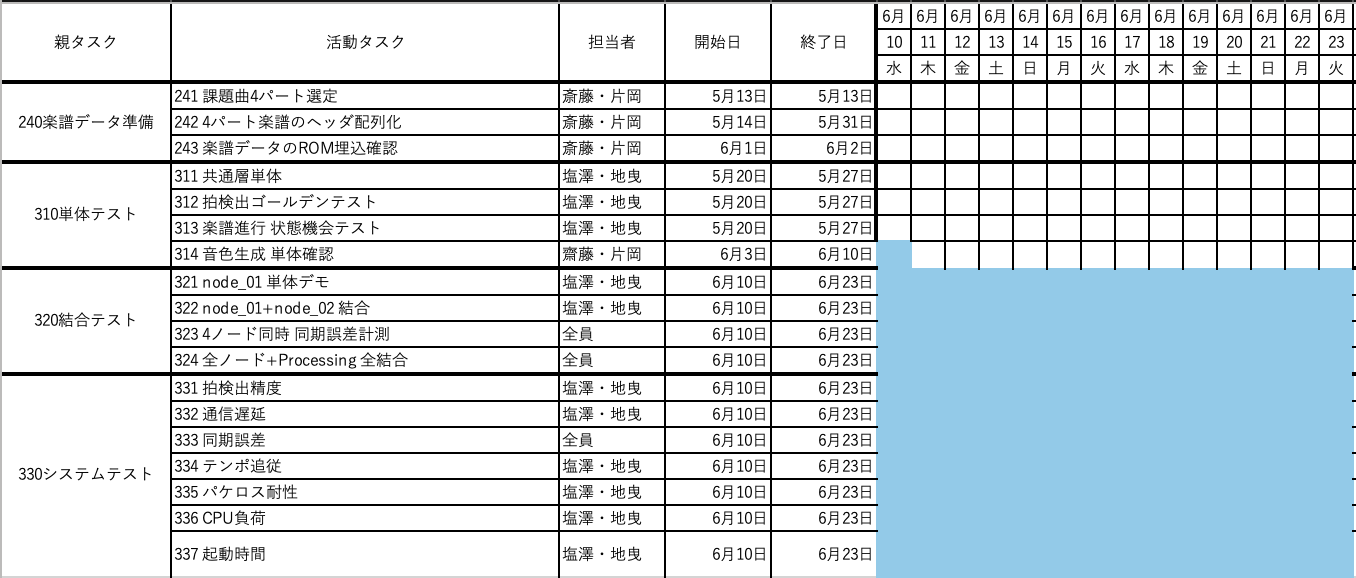
\includegraphics[width=\linewidth]{Figs/before.png}
  \caption{担当箇所のGC（計画前）}
  \label{fig:saito-gc-before}
\end{figure}

\begin{figure}[htbp]
  \centering
  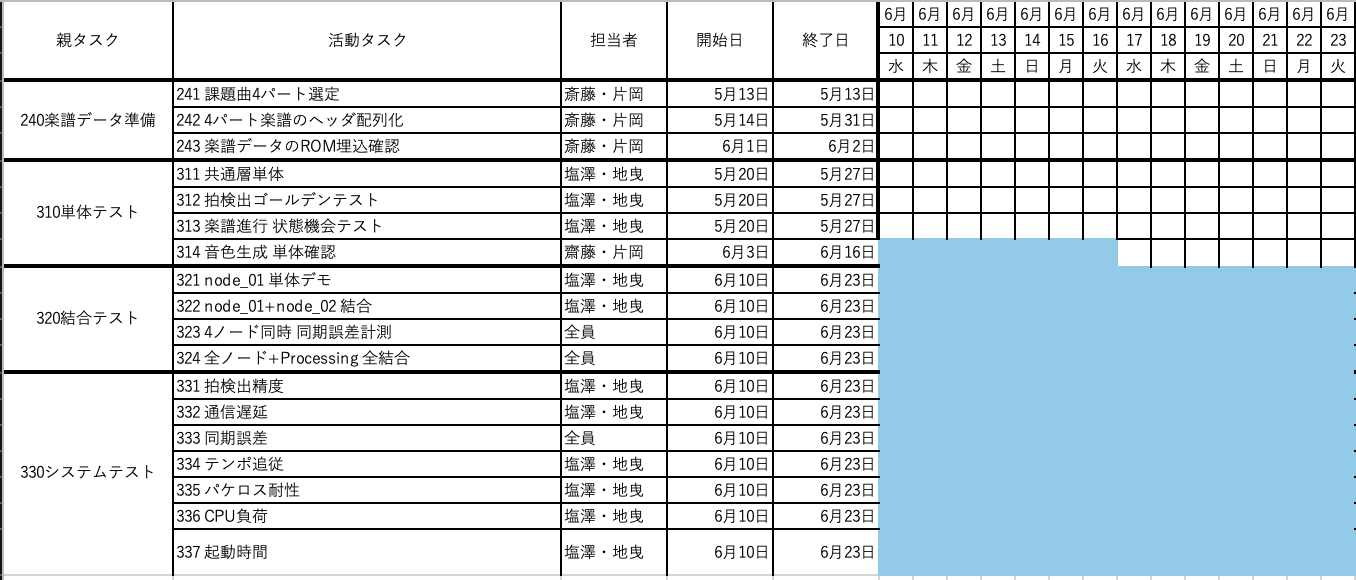
\includegraphics[width=\linewidth]{Figs/after.png}
  \caption{担当箇所のGC（現在）}
  \label{fig:saito-gc-current}
\end{figure}

\sectionrule

\section{課題管理}

{\footnotesize
\renewcommand{\arraystretch}{1.25}
\begin{tabularx}{\linewidth}{@{}>{\raggedright\arraybackslash}p{25mm}X>{\raggedright\arraybackslash}p{11mm}>{\raggedright\arraybackslash}p{11mm}X>{\raggedright\arraybackslash}p{19mm}>{\raggedright\arraybackslash}p{17mm}@{}}
\toprule
課題 & 発生原因 & 影響度 & 優先度 & 対策 & 期限 & 状態 \\
\midrule
なし
  & 現時点で特に大きな課題はない．
  & -- & --
  & --
  & -- & -- \\
\bottomrule
\end{tabularx}
}

\sectionrule

\section{AI利用状況と検証（再現性重視）}

\subsection{利用内容}

\begin{itemize}
  \item 利用目的：音声解析アプリの改良方針整理，トランペット・ドラム音色の調整，作業ログの記載内容整理
  \item 入力（プロンプト要旨）：
    \begin{itemize}
      \item {}前回の金管パートと同じ前提で，ドラムパート作成時に決めるべき内容を確認した．
      \item {}ドラム伴奏を変更する場合の方針として，8拍ごとの区切り，3声がそろう区間，
        終止部の強弱調整について相談した．
      \item {}トランペット音色を改善するため，楽器プロファイル指定，原音アタックの利用，
        薄い金管レイヤー，A/B比較，調整プリセットについて相談した．
      \item {}解析後の各パラメータをスライダーだけでなく数値入力でも変更できるようにする実装を依頼した．
      \item {}作業ログの進捗サマリー，GC，課題管理，AI利用状況の記載内容を
        今回の作業内容に合わせて整理するよう依頼した．
    \end{itemize}
  \item 出力概要：
    \begin{itemize}
      \item {}ドラムパートは基本リズムを維持し，区切りと終止部だけを強調する方針が示された．
      \item {}\texttt{DRUM\_SCORE}のベロシティ調整案と，READMEへ追記する説明文が示された．
      \item {}トランペット音色について，原音に近い，明るく抜ける，太く厚く，ノイズ控えめ，
        金管レイヤー強めの調整プリセット案が示され，解析アプリへ反映された．
      \item {}A/B比較機能と数値入力欄の実装案が示され，ブラウザ上で動作確認した．
      \item {}作業ログの各節について，今回の成果物と未実施項目に合わせた記載案が示された．
    \end{itemize}
\end{itemize}

\sectionrule

\subsection{検証方法}

\begin{itemize}
  \item 検証手法：
    \begin{itemize}
      \item {}AIの出力をそのまま採用せず，リポジトリ内の実ファイル，
        Processingでの確認結果，作業ログの記載内容を照合した．
    \end{itemize}
  \item 参照資料：
    \begin{itemize}
      \item なし
    \end{itemize}
  \item 検証手順：
    \begin{enumerate}
      \item {}\texttt{DRUM\_SCORE}に8拍ごとの区切り，3声がそろう区間，
        終止部の強弱調整が反映されていることを確認した．
      \item {}Processing上で金管3声，チューバ低音，ドラム伴奏を再生し，
        音量バランスと終止部の聞こえ方を確認した．
      \item {}解析アプリをブラウザで起動し，A/B比較，調整プリセット，数値直接入力が動作することを確認した．
      \item {}変更後GCの図が作業ログの第3節から参照されていることを確認した．
    \end{enumerate}
\end{itemize}

\sectionrule

\subsection{ファクトチェック結果}

\begin{itemize}
  \item 一致点：
    \begin{itemize}
      \item {}\texttt{kaeru\_score\_debug.pde}に，金管3声，チューバ低音，
        ドラム伴奏の\texttt{ScoreEvent}配列が存在することを確認した．
      \item {}ドラムパートの強弱調整と，READMEの説明が対応していることを確認した．
      \item {}金管楽器の音色データが存在し，Processing確認用スケッチで読み込まれていることを確認した．
      \item {}音声解析アプリに，A/B比較機能，調整プリセット，数値直接入力欄が追加されていることを確認した．
      \item {}変更後GCが第3節の現在GCとして掲載されていることを確認した．
    \end{itemize}
  \item 不一致・疑義：
    \begin{itemize}
      \item {}Processing上での確認は実施済みである一方，
        Arduinoファームウェアへの反映と実機確認は未実施である．
      \item {}ドラム伴奏とドラム音色の分析・作成は完了しているが，
        曲中での自然さを高めるための微調整は未完了である．
      \item {}トランペット音色は解析アプリ上で調整しやすくなったが，
        最終的に採用する音色は楽曲内で聞き比べて決める必要がある．
    \end{itemize}
  \item 最終判断：
    \begin{itemize}
      \item {}Processingで確認済みのドラム伴奏作成は今回の成果として記載し，
        Arduino側への反映・実機確認を今後の課題として記載する．
      \item {}ドラム音色については分析・作成済みの成果として記載し，
        微調整を今後の課題として記載する．
      \item {}トランペット音色の調整UI改善は今回の成果として記載し，
        最終採用音色の決定を次回作業として記載する．
    \end{itemize}
  \item 根拠：
    \begin{itemize}
      \item {}Processing確認用スケッチ，README，変更後GC，作業ログ本文を照合した結果による．
    \end{itemize}
\end{itemize}

\sectionrule

\section{次回計画}

\begin{itemize}
  \item 目標：
    \begin{itemize}
        \item {}作成した楽譜データをArduino側の統合作業へ受け渡す．
    \end{itemize}
  \item 達成基準：
    \begin{itemize}
      \item {}統合後の楽譜データについて，ROM埋込確認を実施できる状態になっている．
    \end{itemize}
  \item 期限：
    \begin{itemize}
      \item {}次回打合せまたはファームウェア統合作業の開始前
    \end{itemize}
\end{itemize}

\sectionrule


\section{付録}

\begin{itemize}
  \item 添付資料：
    \begin{itemize}
      \item ソースコード：\texttt{https://github.com/takushio2525/2026-hackathon-team23}
    \end{itemize}
  \item 添付範囲：
    \begin{itemize}
      \item 今回の確認対象である楽譜データおよび試聴確認用成果物の全体
    \end{itemize}
\end{itemize}

\sectionrule

\end{document}
